\documentclass[a4paper,12pt]{article} 
\usepackage[left=2.5cm,right=1cm,top=2.5cm,bottom=2cm]{geometry}
%%% Работа с русским языком
\usepackage{cmap}					% поиск в PDF
%\usepackage{mathtext} 				% русские буквы в фомулах
\usepackage[T2A]{fontenc}			% кодировка
\usepackage[utf8]{inputenc}			% кодировка исходного текста
\usepackage[english,russian]{babel}	% локализация и переносы
\usepackage{amsmath} 
\usepackage{float}
\usepackage{graphicx}
\graphicspath{ {./images/} }
\usepackage{hyperref}
\hypersetup{				% Гиперссылки
    unicode=true,           % русские буквы в раздела PDF
    colorlinks=true,        % false: ссылки в рамках; true: цветные ссылки
    linkcolor=black,        % внутренние ссылки
    citecolor=black,        % на библиографию
    filecolor=magenta,      % на файлы
    urlcolor=blue           % на URL
}

% \usepackage{tocbasic}
% \renewcommand*{\listoffigures}{\listoftoc[\listfigurename]{lof}}
% \renewcommand*{\listoftables}{\listoftoc[\listtablename]{lot}}
% % \setuptoc{lof}{leveldown,totoc}
% % \setuptoc{lot}{leveldown,totoc}

%%% Дополнительная работа с математикой
\usepackage{amsmath,amsfonts,amssymb,amsthm,mathtools} % AMS
\usepackage{icomma} % "Умная" запятая: $0,2$ --- число, $0, 2$ --- перечисление

%% Номера формул
%\mathtoolsset{showonlyrefs=true} % Показывать номера только у тех формул, на которые есть \eqref{} в тексте.

\usepackage{cite} % Работа с библиографией
%\usepackage[superscript]{cite} % Ссылки в верхних индексах
%\usepackage[nocompress]{cite} % 
\usepackage{csquotes} % Еще инструменты для ссылок


\begin{document} % конец преамбулы, начало документа
%\pagestyle{empty} 
\thispagestyle{empty}

\begin{center}
    {\huge
    Частное общеобразовательное учреждение
    
    <<Школа разговорных языков>>
    }
    \vfill
    \vfill
    \vfill
    \vfill
    {\huge \textsc{ПРОЕКТ}}
    \vfill
    {\huge на тему}
    \vfill
{\huge \textsc{\textbf{«Конъюнкция и Исключающее ИЛИ.}}}

\vspace{0.5cm}

{\huge \textsc{\textbf{Демонстрация логических функций на стенде»}}}
\vfill
{\huge (по Информатике и ИКТ)}

\vfill 
    
    \begin{flushright}
    {\Large ученика 10 класса 
    
    \vspace{0.5cm}

    Доричева Тимофея Константиновича}
    \end{flushright}
    \vfill
    {\Large Санкт-Петербург
    
    \vspace{0.5cm}

    2023}
\end{center}
\pagebreak

\tableofcontents

\section{Введение}

Цель данного проекта~--- наглядно пояснить суть некоторых логических (б\'{у}левых\footnote{Булевы функции названы в честь Джорджа Буля (1815—1864), английского математика и логика.}) функций, а~именно конъюнкции и исключающего ИЛИ, и~продемонстрировать их на стенде, собранном на макетной плате. Работа оформлена в~издательской системе \LaTeX.


\section{Логические функции}

Б\'{у}лева функция (или логическая функция, или функция алгебры логики) от $n$~аргументов~--- в~дискретной математике~--- отображение вида


\begin{align}\label{eq:BnB}
 B^n \rightarrow B
\end{align}

где $B = \{0,1\}$ — булево множество. 

Неотрицательное целое число $n$, обозначающее количество аргументов, называется \textit{арностью} функции. Так, для $n = 2$ имеем бинарные функции, т.е. функции двух аргументов:

\begin{align}\label{eq:B2B}
 B^2 \rightarrow B
\end{align}

или

\begin{align}\label{eq:BBB}
B \times B \rightarrow B
\end{align}

Ниже рассмотрим два примера бинарных логических функций.

\subsection{Конъюнкция}

Конъ\'{ю}нкция (от лат. \textit{conjunctio}~--- «союз, связь»)~--- логическая операция, по смыслу максимально приближенная к союзу «и». Синонимы: логическое «И», логическое умножение, иногда просто «И».

Суть конъюнкции~--- результатом является истина тогда и только тогда, когда все аргументы (оба для бинарной функции) истинны, иначе~--- ложь, см. рис.~\ref{and} и табл.~\ref{AND_table}.

\begin{figure}[h]
    \begin{center}
    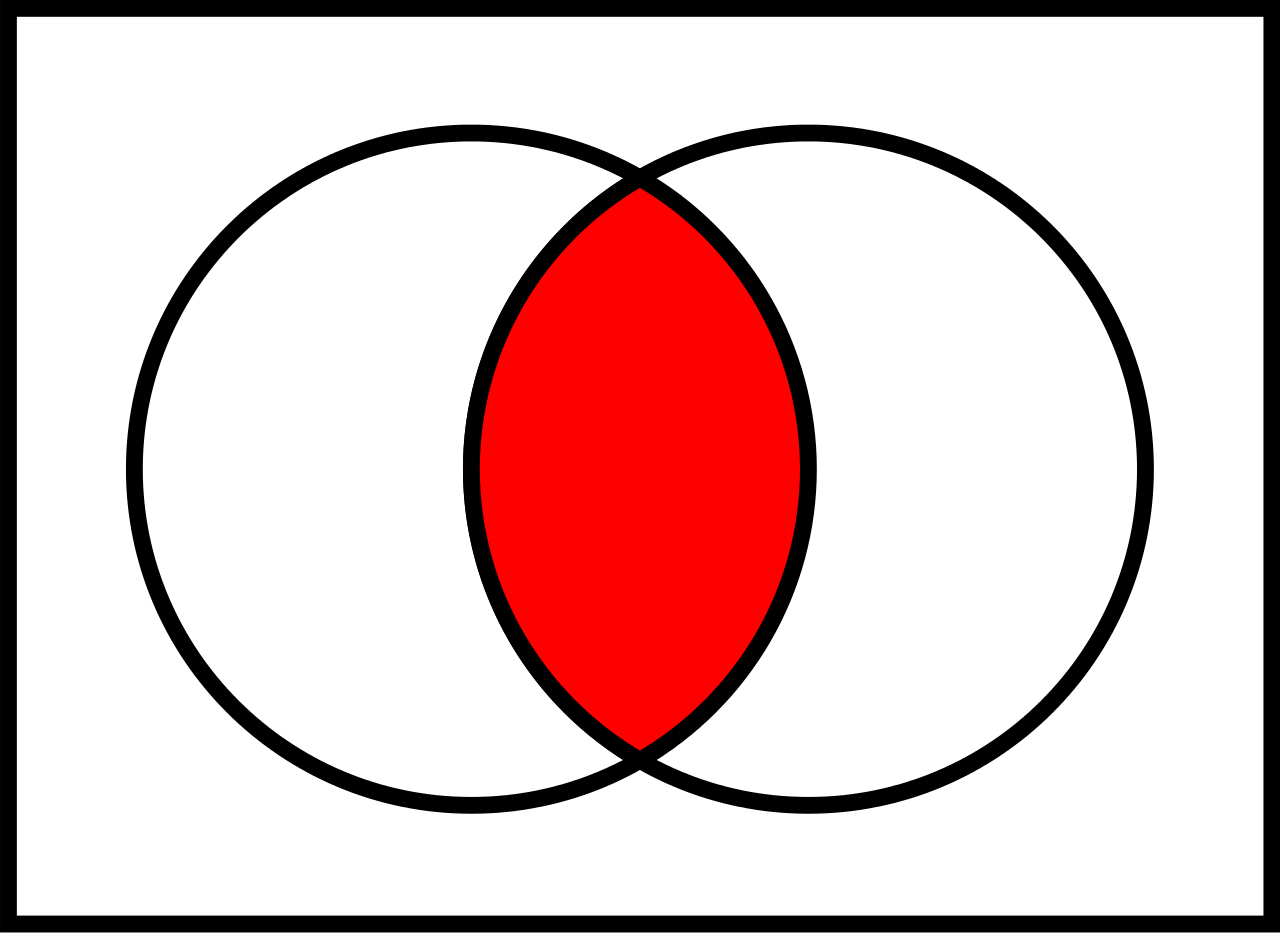
\includegraphics[width=5cm]{and}    
    \caption{Конъюнкция. Диаграмма Эйлера — Венна}
    \label{and}
    \end{center}
\end{figure}


\begin{table}[h!]
    \caption{Логическая функция И. Таблица истинности.\label{AND_table}}
    \begin{center}
    \begin{tabular}{||c c c||} 
     \hline
     A & B & Y \\ [0.5ex] 
     \hline\hline
     0 & 0 & 0 \\ 
     \hline
     0 & 1 & 0 \\
     \hline
     1 & 0 & 0 \\
     \hline
     1 & 1 & 1 \\ 
     \hline
    \end{tabular}
    \end{center}
\end{table}

\subsection{Исключающее ИЛИ}

Исключ\'{а}ющее «или» (сложение по модулю 2, XOR) — булева функция, а~также логическая и~битовая операция. В~случае двух переменных результат выполнения операции истинен тогда и~только тогда, когда один из аргументов истинен, а другой — ложен, см.~рис.~\ref{xor} и~табл.~\ref{XOR_table}.

\begin{figure}[h]
    \begin{center}
    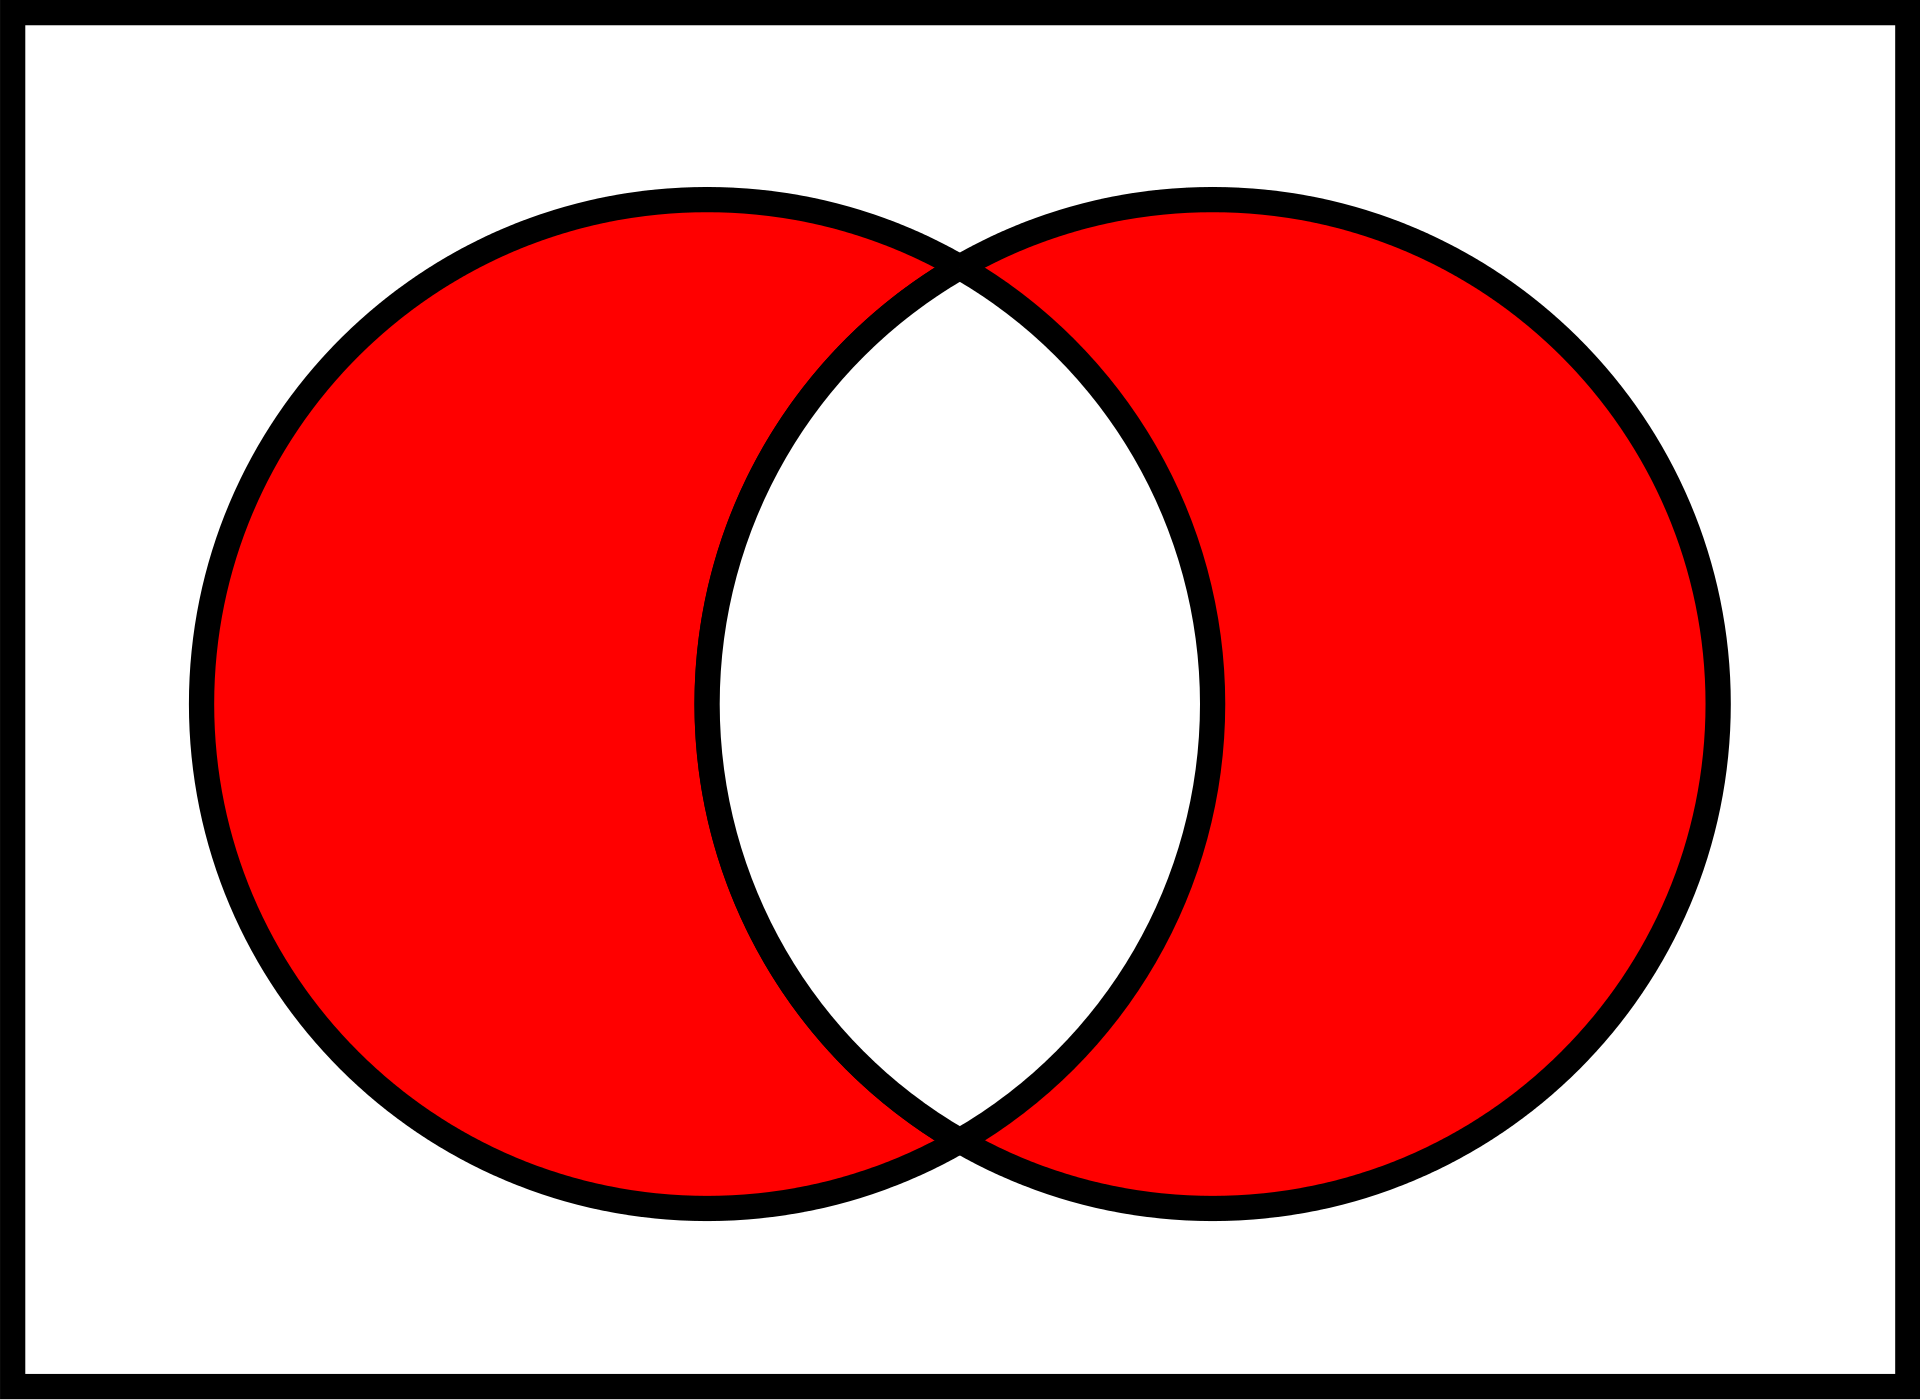
\includegraphics[width=5cm]{xor}    
    \caption{Исключающее ИЛИ. Диаграмма Эйлера — Венна}
    \label{xor}
    \end{center}
\end{figure}

\begin{table}[h!]
    \caption{Логическая функция Исключающее ИЛИ. Таблица истинности.\label{XOR_table}}
    \begin{center}
    \begin{tabular}{||c c c||} 
     \hline
     A & B & Y \\ [0.5ex] 
     \hline\hline
     0 & 0 & 0 \\ 
     \hline
     0 & 1 & 1 \\
     \hline
     1 & 0 & 1 \\
     \hline
     1 & 1 & 0 \\ 
     \hline
    \end{tabular}
    \end{center}
\end{table}

\section{Демонстрационный стенд}

Демонстрационный стенд собран на макетной плате и содержит:
\begin{itemize}
    \item Общую часть
    \item Конъюнктор
    \item Исключающее ИЛИ
    \item Блок питания
\end{itemize}

Общий вид стенда показан на рис.~\ref{general_view}.

Электропитание осуществляется от блока питания напряжением 5~В.

В левой части платы собрана общая часть и конъюнктор. В правой части платы, отделённой на рис.~\ref{general_view} наклонной чертой,~--- исключающего ИЛИ. 

Общая часть содержит кнопки для подачи высоких сигналов на входы и индицирующие эти сигналы светодиоды жёлтого и зелёного цвета.

\begin{figure}[h]
    \begin{center}
    \label{general_view}
    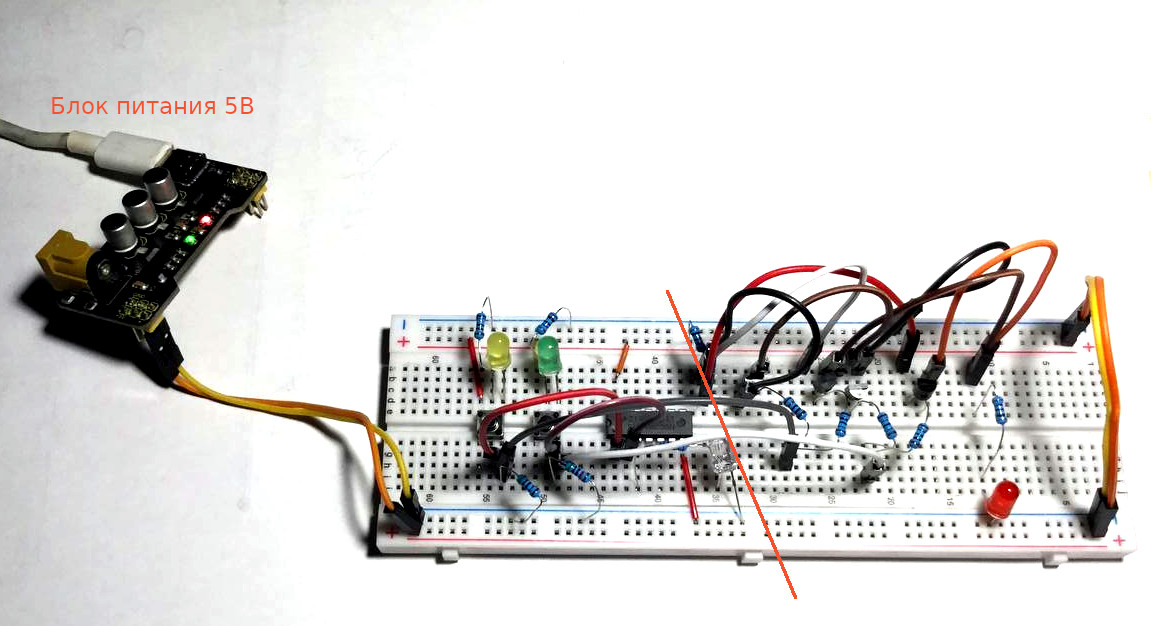
\includegraphics[width=\textwidth]{general_view}    
    \caption{Демонстрационный стенд. Общий вид.}
    \end{center}
\end{figure}

Светодиод белого цвета ~--- суть результат функции И.

Схема исключающего ИЛИ собрана в правой части платы, см. рис.~\ref{general_view} и реализована на транзисторах.

Светодиод красного цвета ~--- суть результат функции исключающее ИЛИ.

Функция И реализована на микросхеме SNx4HC08. Состав микросхемы показан на рис.~\ref{SNx4HC08}.

\begin{figure}[h]
    \begin{center}
    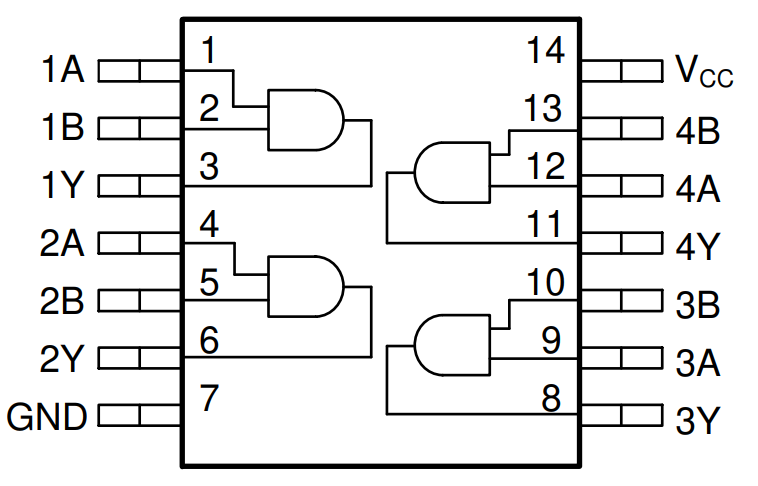
\includegraphics[width=5cm]{SNx4HC08}    
    \caption{Микросхема SNx4HC08. Назначение выводов.}
    \label{SNx4HC08}
    \end{center}
\end{figure}



\section{Демонстрация работы}

Для демонстрации работы стенда будем поочередно подавать на входы сигналы из табл.~\ref{AND_table} и контролировать выход по белому и красному светодиодам.

\subsection{Входные сигналы 0,0}

Не горят ни жёлтый, ни зелёный светодиоды. Не горят ни красный, ни белый светодиоды. См. рис.~\ref{general_view} и таблицы \ref{AND_table},~\ref{XOR_table}.

\subsection{Входные сигналы 0,1}

Горит только зелёный светодиод. Горит только красный светодиод. См. рис.~\ref{state01} и таблицы \ref{AND_table},~\ref{XOR_table}.

\begin{figure}[H]
    \begin{center}
    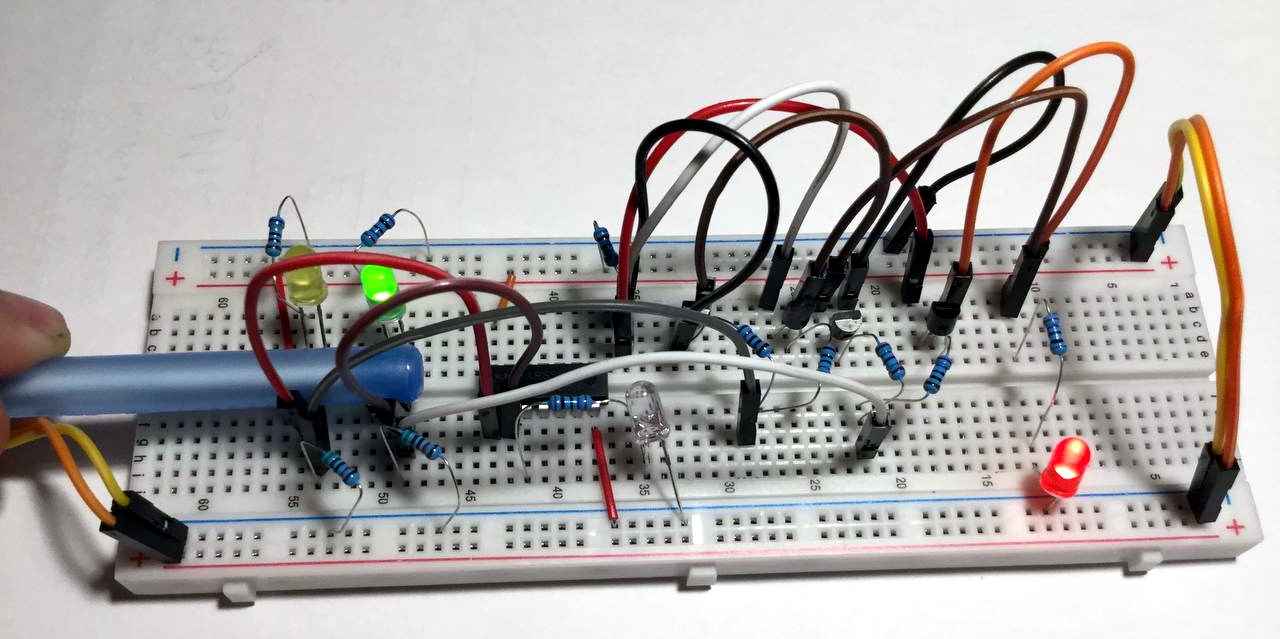
\includegraphics[width=\textwidth]{state01}    
    \caption{Входные сигналы 0, 1.}
    \label{state01}
    \end{center}
\end{figure}

\subsection{Входные сигналы 1,0}

Горит только жёлтый светодиод. Горит только красный светодиод. См. рис.~\ref{state10} и таблицы \ref{AND_table},~\ref{XOR_table}.

\begin{figure}[H]
    \begin{center}
    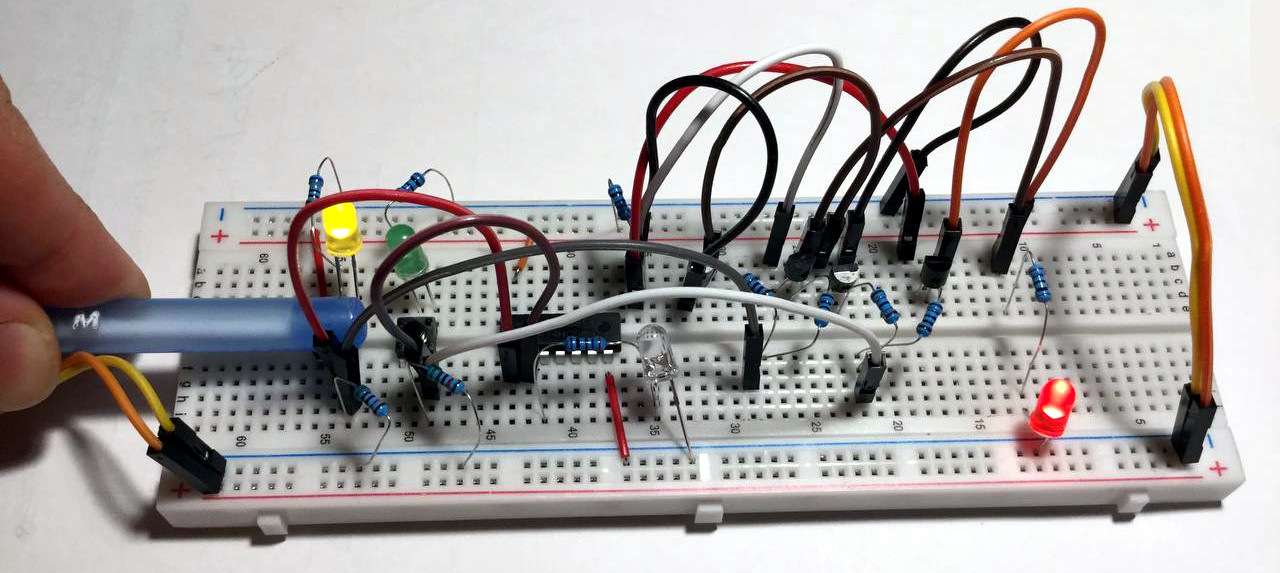
\includegraphics[width=\textwidth]{state10}    
    \caption{Входные сигналы 1, 0.}
    \label{state10}
    \end{center}
\end{figure}

\subsection{Входные сигналы 1,1}

Горят оба светодиода жёлтый и зелёный. Горит белый светодиод и не горит красный светодиод. См. рис.~\ref{state11} и таблицы \ref{AND_table},~\ref{XOR_table}.

\begin{figure}[H]
    \begin{center}
    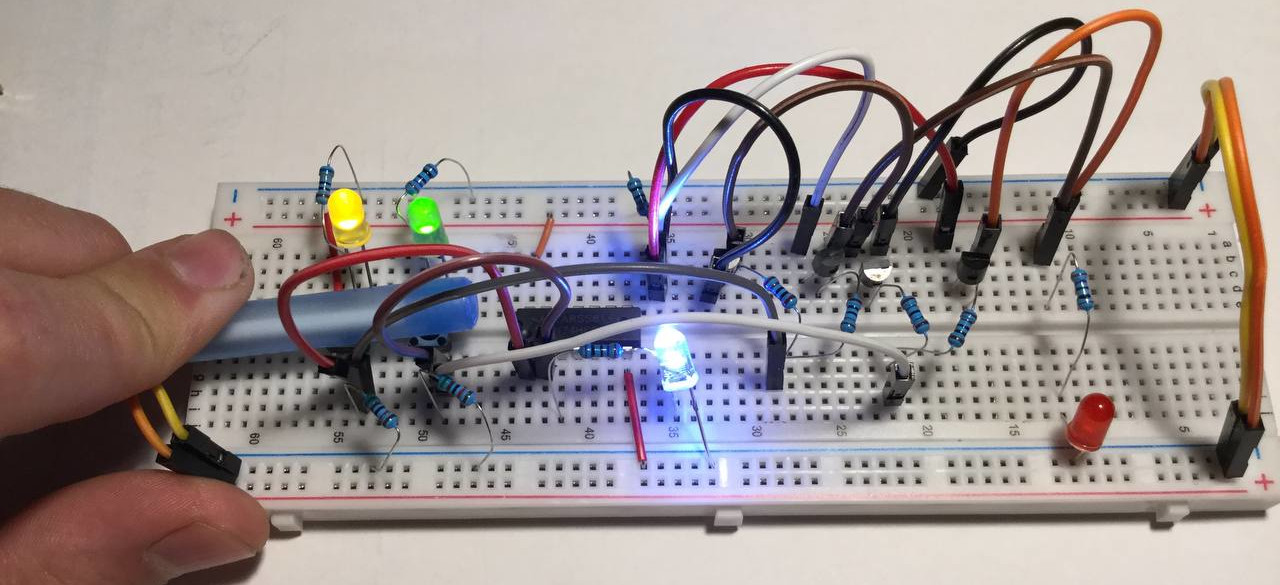
\includegraphics[width=\textwidth]{state11}    
    \caption{Входные сигналы 1, 1.}
    \label{state11}
    \end{center}
\end{figure}


\section{Заключение}

Этот проект наглядно паказывает, что электроника~--- это несложно и интересно.  

\addcontentsline{toc}{section}{Список иллюстраций}

\listoffigures

\addcontentsline{toc}{section}{Список таблиц}
\listoftables

\begin{thebibliography}{9}
    \addcontentsline{toc}{section}{\refname}
    \bibitem{}Чарльз Платт: Электроника для начинающих.~--- СПб.: БХВ, 2021.~--- 416~с.: ил.
    \bibitem{sn74hc08}SNx4HC08 Quadruple 2-Input AND Gates. Datasheet~--- Texas Instruments, 2021.~--- 34~с.: \url{www.ti.com}
\end{thebibliography}

\end{document}
